%!TEX TS-program = pdflatex
%!TEX root = i3det-top.tex
%!TEX encoding = UTF-8 Unicode

\section{Introduction}
\label{sec:intro}

% \subsection{IceCube Science}
Construction of an observatory to examine celestial phenomena using
neutrinos was first conceived not long after Pauli first theorized the
particle's existence.  In the six decades following the experimental
discovery of the neutrino by Cowan and Reines, detectors have been realized
that have steadily progressed toward the goal of multimessenger neutrino
astronomy.  Early developments in the field include the first detections of
atmospheric neutrinos in deep underground telescopes \cite{Witwatersrand,KGF} and
radiochemical neutrino detectors characterizing the flux of neutrinos from
nuclear fusion in the Sun \cite{Homestake, GALLEX}. A handful of neutrino
events were detected from supernova SN1987A
\cite{SK1987A,IMB1987A,BUST1987A}, providing the first glimpse of neutrino
from outside the solar system.  Advanced
atmospheric and solar neutrino observatories provided definitive
evidence of neutrino mass and constrained neutrino mixing
parameters \cite{SK,SNO}.  The study of neutrinos emanating from astrophysical
processes has both informed and sometimes surprised the fields of
astrophysics and particle physics. 

Notwithstanding the events seen from SN1987A, a remarkable but
extremely rare class of phenomena, the detection of neutrinos originating in
astrophysical processes outside our solar system requires detector facilities of
extreme dimensions to detect the faint fluxes of these weakly-interacting
particles.  The motivations for such massive observatories are numerous, however.
Neutrinos, because of their weak neutral character, are useful probes of high
energy phenomena in the Universe. Unlike photons, their origins in astrophysical
acceleration sites unambiguously point to hadronic acceleration and
provide identification of the origins of cosmic rays. They arrive upon detection
undeflected and unscattered and thus point back to their originators and provide
a clear view of the physics deep within shrouded and compact sources. At extreme
energies of several PeV and above, they are the only particles which can reach 
us from sources at cosmological distances.

Progress toward large-scale neutrino observatories using arrays of
photomultiplier tubes in water or ice was achieved through the efforts of
DUMAND \cite{DUMAND}, AMANDA \cite{AMANDA:detector}, Baikal \cite{Baikal}, and
ANTARES \cite{ANTARES}.  These experiments provided key measurements of the
high-energy atmospheric neutrino spectrum, constrained optimistic models of
astrophysical neutrino production, and demonstrated the feasibility of the
technique. However, the detection of astrophysical neutrinos proved
elusive, suggesting that a kilometer-scale array was required to achieve the necessary sensitivity.  

The primary mission of the IceCube Neutrino Observatory has 
been the discovery of astrophysical neutrinos, achieved in 2013 \cite{IC3:evidence}, and 
idenfitication and characterization of the sources.  Other diverse science
objectives include detection of dark matter and other exotic particles,
studies of neutrino oscillation physics, and detection of the neutrino shockwave
from a Galactic core-collapse supernova.  A robust multi-messenger collaboration
with optical, gamma-ray, radio, and gravitational wave observatories
provides multiple windows on the potential neutrino sources.  A key to
the success of these initiatives is the reliability and performance of the
IceCube instrumentation, as well as the flexibility and stability of the
online software systems.  

\subsection{A Functional Description of the IceCube Instrument}

In order to observe astrophysical neutrinos, the primary science goal of the
experiment, IceCube exploits the fact that charged particles moving through the
ice at super-luminal speed emit Cherenkov photons. An enormous detection volume
is required due to the small cross-sections of neutrinos for producing
secondary charged particles in interactions with ordinary matter. The glacial
ice cap at the South Pole is about \SI{3}{\kilo\meter} thick and is an ideal
operational site, since it not only offers a large quantity of interaction
material but also a medium with excellent optical qualities.  With a
Cherenkov photon yield of $\mathcal{O}(\num{E5})$ visible photons per
\SI{}{\giga\electronvolt} of secondary particle shower energy, the long
optical attenuation length of South Pole ice, and large-area
photomultipliers (PMTs), it is possible to instrument cubic kilometers of
ice with a rather sparse spacing of detectors.

The basic detection unit in IceCube in order to capture the Cherenkov light is the
digital optical module (DOM), covered in detail in Sec.~\ref{sec:dom}.
Encapsulated in a \SI{1/2}{''} thick glass pressure sphere 
to withstand the extreme pressure in the deep ice, the main components of a DOM
are a \SI{10}{''} PMT, embedded high-voltage generation, a flasher calibration
board, and a mainboard containing the analog and digital processing circuitry
for PMT pulses.  The transmission of the digital data is controlled by an FPGA
and embedded processor hosted on the mainboard. The digitized data is sent to a
central computing facility at the surface via a cable system described in
Sec.~\ref{sec:cable}.  Aspects of detector deployment and ice drilling are
covered in Sec.~\ref{sec:drill-deploy}. An overview of the data flow as well as
its readout, processing and filtering are presented in
Sec.~\ref{sec:online}, along with data handling, monitoring, and operational performance of
the observatory. The IceCube instrument consists of three sub-detectors ---
IceCube, DeepCore, and IceTop --- using the same instrumentation design of
DOMs and associated surface readout. A schematic layout of the array is
shown in Fig.~\ref{fig:array}. 

\begin{figure}[!h]
 \centering
 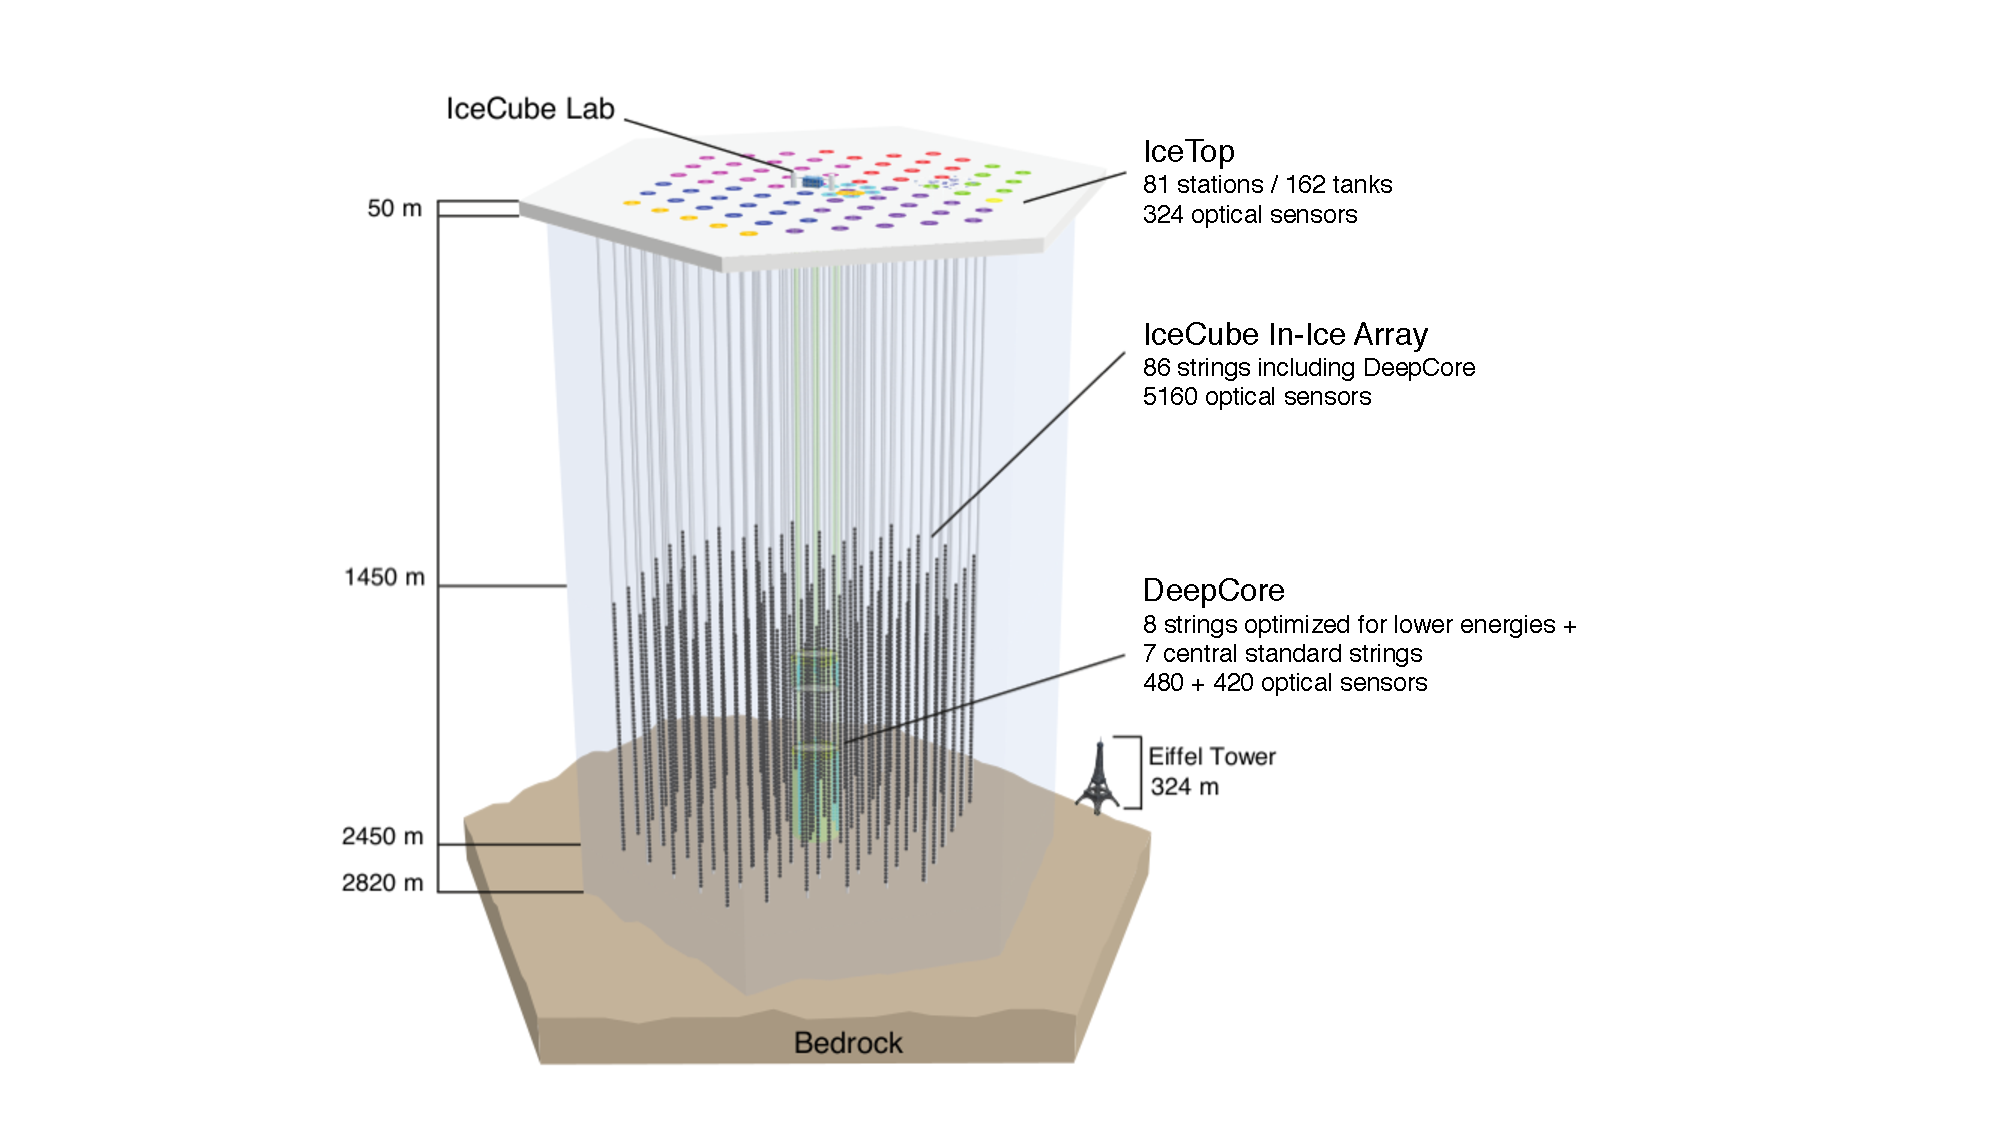
\includegraphics[width=0.8\textwidth]{graphics/intro/ArrayWSeasonsLabels_crop.pdf}
 \caption{The IceCube Neutrino Observatory with its sub-array DeepCore and
   the cosmic ray air shower array IceTop.}
 \label{fig:array}
\end{figure}

\subsubsection{IceCube}

In order to detect the Cherenkov photons emitted by charged particles
traversing the ice, \num{5160} DOMs are deployed between \SI{1450}{\meter}
and \SI{2450} {\meter} below the glacial surface on \num{86} vertical
strings, with each string consisting of \num{60} DOMs deployed along a copper cable. The
primary in-ice array consists of \num{78} strings with a vertical
separation of the DOMs of \SI{17}{\meter}.  The strings are
deployed on a hexagonal grid with \SI{125}{\meter} horizontal spacing that
spans a volume of one cubic kilometer of ice.  This design was chosen in
order to meet the primary science requirement of detecting astrophysical
neutrinos in the energy range of $\mathcal{O}(\SI{}{\tera\electronvolt})$--
$\mathcal{O}(\SI{}{PeV})$.  % The observation of these neutrinos was achieved
% by searching for events that start inside the volume of IceCube and deposit
% more than \SI{30}{\tera\electronvolt} of energy \cite{IC3:evidence}. 

Two different event topologies form the standard signatures of neutrinos in
IceCube.  Track-like events originate from a charged current interaction of
a high-energy muon neutrino with a nucleus, producing a hadronic cascade at
the vertex and an outgoing muon that emits a Cherenkov cone along its
track.  The angular reconstruction of such a muon track and hence the
incident neutrino direction can reach a resolution better than
$\SI{1}{\degree}$, confirmed by analysis of the Moon shadow
\cite{IC3:moon}. Energy loss above the minimum-ionizing regime, typically $ \sim
\SI{1}{\tera\electronvolt}$ in IceCube, is dominated by stochastic
processes resulting in large fluctuations in the amount of energy deposited
for different muons of the same energy.  A second class of events are
electromagnetic or hadronic cascades from interactions of all neutrino
flavors, resulting in a more spherical light deposition in the detector.
Since the total light output of such a cascade is directly proportional to its energy, and
the cascades are often well-contained in the detector, the neutrino energy
reconstruction for such events is much more precise than for track-like
events. The average deposited energy resolution for both event types
combined is $ \sim \SI{15}{\%}$ \cite{IC3:ereco}.

\subsubsection{DeepCore}

A subset of in-ice DOMs is deployed in the deep ice below a
depth of \SI{1750}{\meter} with a denser instrumented volume and
correspondingly lower energy threshold. This
sub-array, DeepCore \cite{ICECUBE:DC}, consists of eight specialized and
closely-spaced strings of sensors in the center of the array, along with
the seven standard central IceCube strings.  The average inter-string
spacing of 13 of 15 of the strings is \SI{72}{\meter}, with six of the 15
spaced at \SI{42}{\meter}.

The eight specialized DeepCore strings have a DOM-to-DOM spacing of
\SI{7}{\meter} for the bottom 50 DOMs, deployed at depths of
\SI{2100}{\meter} and \SI{2450}{\meter}.  The remaining 10 DOMs are
deployed at depths above \SI{2000}{\meter} with a spacing of
\SI{10}{\meter} to form a veto cap, allowing better rejection of downgoing
atmospheric muons.  Depths from \SI{2000}{\meter} to \SI{2100}{\meter}
is not instrumented, as it is a region in the ice of significantly
increased optical scattering and absorption (the ``dust layer'').

Six of the DeepCore strings are fully populated with
DOMs using PMTs with \SI{35}{\%} higher quantum efficiency than the
standard IceCube modules.  The denser geometry and increased efficiency
result in a lower energy threshold of about \SI{10}{\giga\electronvolt}.  The design
is optimized for the detection of atmospheric neutrinos with energies
from \SI{10}{\giga\electronvolt} to \SI{400}{\tera\electronvolt}
\cite{ICECUBE:AtmNu}. 

\subsubsection{IceTop}

The air shower array IceTop \cite{ICECUBE:IceTop} consists of \num{81}
Cherenkov tanks filled with clear ice and arranged in pairs on the
surface, using approximately the same grid on which the in-ice
array is deployed.  The two tanks at each surface station are separated from
each other by \SI{10}{\meter}. Each tank contains two standard IceCube
DOMs, one ``high-gain'' DOM operated at a PMT gain of $5 \times 10^{6}$, and one
``low-gain'' DOM operated at a gain of $10^{5}$. Air showers initiated in the atmosphere by cosmic rays are typically
spread over a number of stations. The light generated in the tanks by the
shower particles (electrons, photons, muons and hadrons) is a measure of
the energy deposition of these particles in the tanks. IceTop is sensitive to
primary cosmic rays of energies in the range of \SI{}{PeV} to \SI{}{EeV}
with an energy resolution of \SI{25}{\%} at \SI{2}{PeV}, improving to
\SI{12}{\%} above \SI{10}{PeV} \cite{IT:measurement}.




